\documentclass{standalone}
\usepackage{tikz}
\usetikzlibrary{patterns, positioning}
\usepackage[sfdefault]{ClearSans} %% option 'sfdefault' activates Clear Sans as the default text font
\usepackage[T1]{fontenc}

\begin{document}
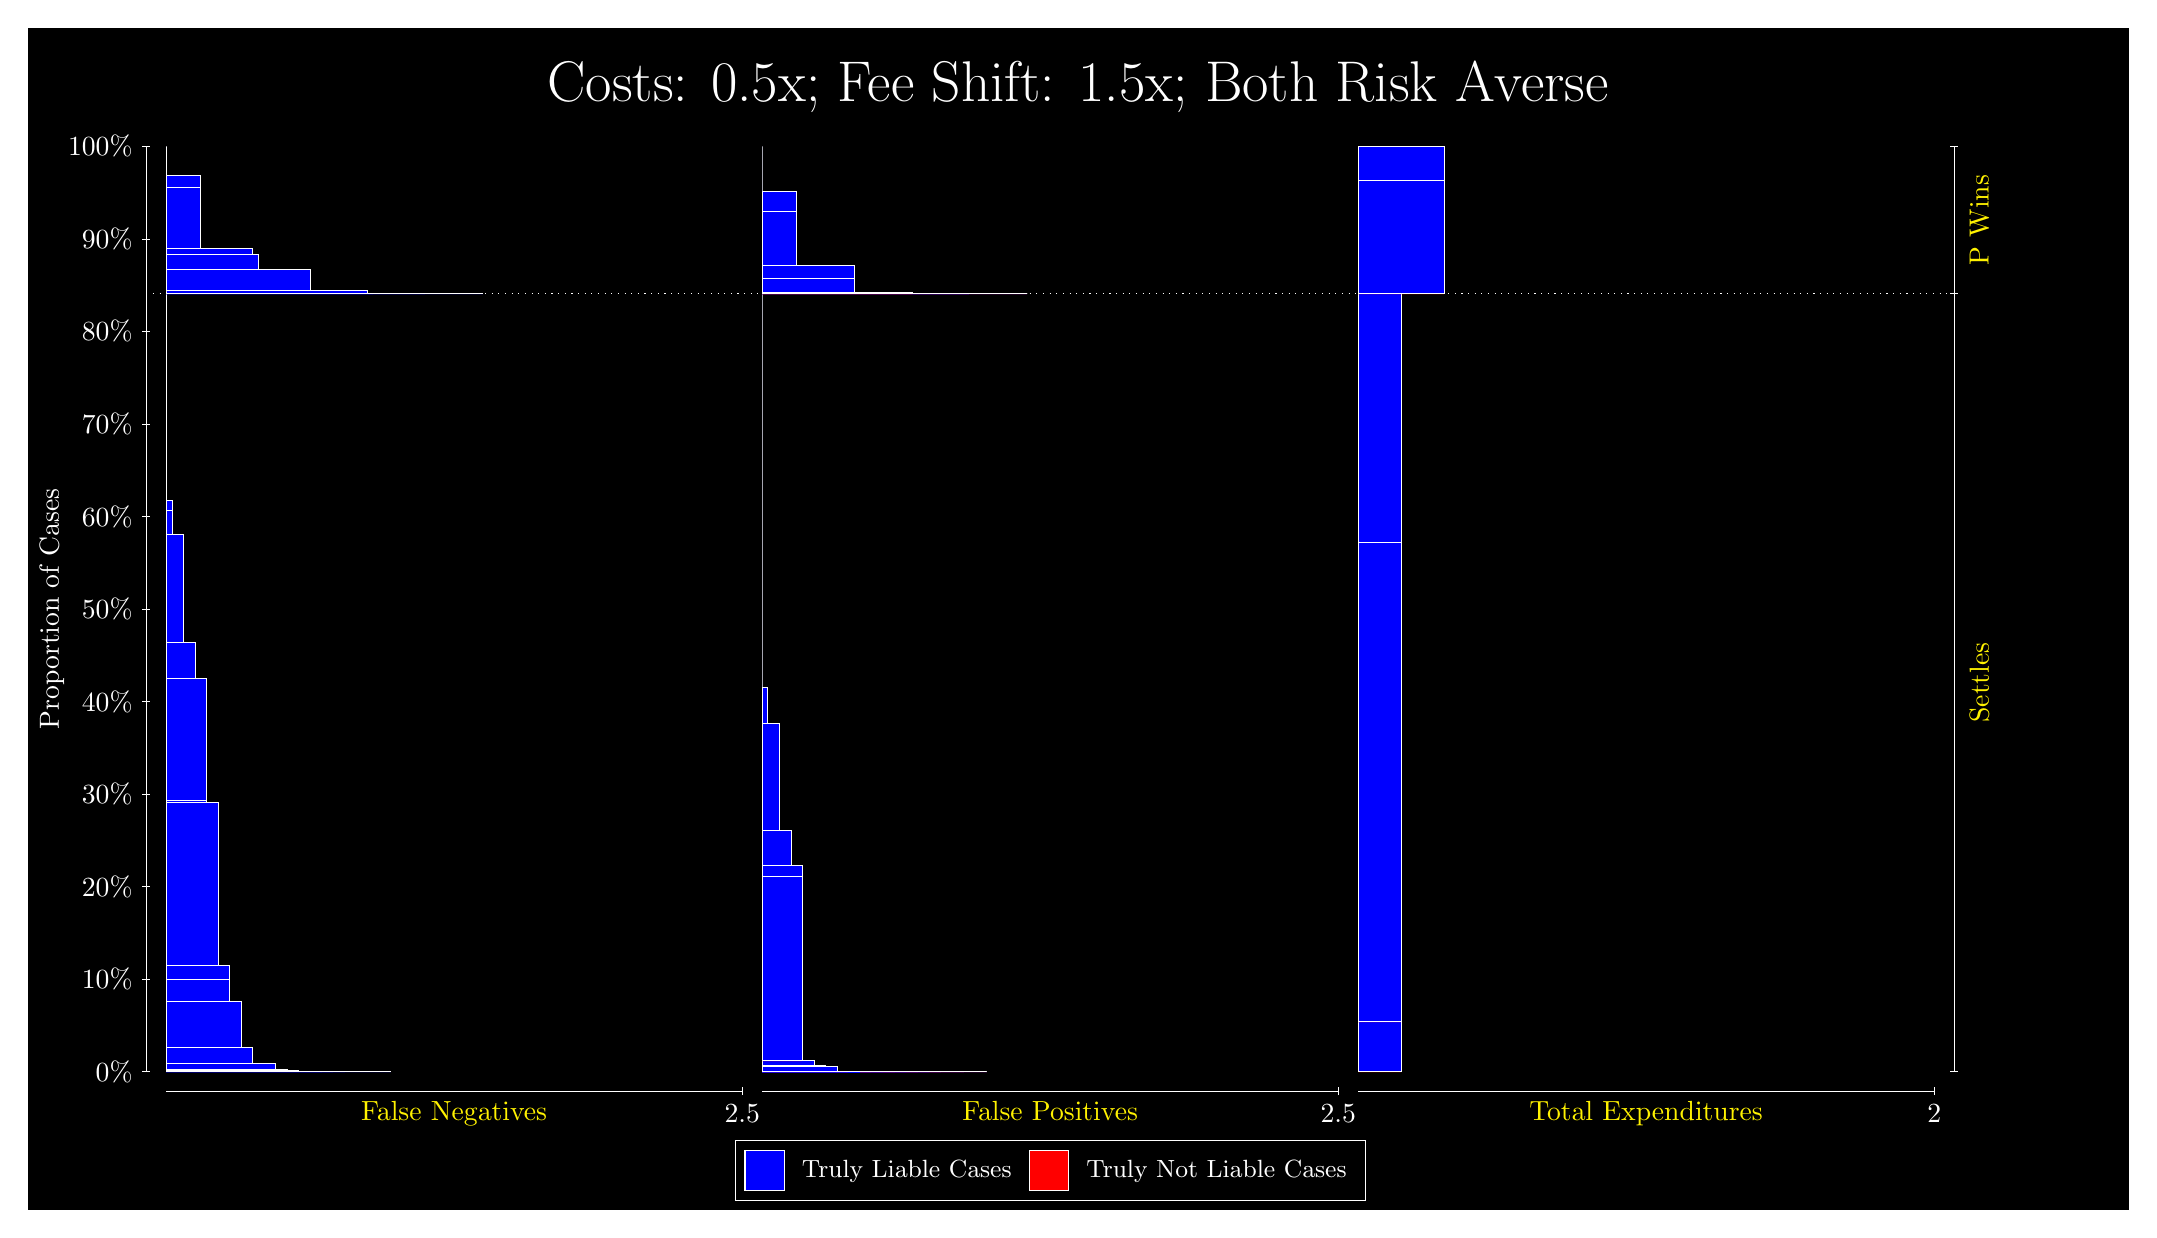
\begin{tikzpicture}
\draw[fill=black] (0,0) rectangle (26.667,15);
\draw[text=white] (0,13.5) rectangle (26.667,15) node[midway] {\huge Costs: 0.5x; Fee Shift: 1.5x; Both Risk Averse};
\draw[white, very thin] (1.5,1.75) -- (1.5,13.5);
\node[rotate=90, text=white, anchor=center] at (0.3, 7.625) {Proportion of Cases};
\draw[white, very thin] (1.45,1.75) -- (1.55,1.75);
\node[text=white, anchor=east] at (1.45, 1.75) {0\%};
\draw[white, very thin] (1.45,2.925) -- (1.55,2.925);
\node[text=white, anchor=east] at (1.45, 2.925) {10\%};
\draw[white, very thin] (1.45,4.1) -- (1.55,4.1);
\node[text=white, anchor=east] at (1.45, 4.1) {20\%};
\draw[white, very thin] (1.45,5.275) -- (1.55,5.275);
\node[text=white, anchor=east] at (1.45, 5.275) {30\%};
\draw[white, very thin] (1.45,6.45) -- (1.55,6.45);
\node[text=white, anchor=east] at (1.45, 6.45) {40\%};
\draw[white, very thin] (1.45,7.625) -- (1.55,7.625);
\node[text=white, anchor=east] at (1.45, 7.625) {50\%};
\draw[white, very thin] (1.45,8.8) -- (1.55,8.8);
\node[text=white, anchor=east] at (1.45, 8.8) {60\%};
\draw[white, very thin] (1.45,9.975) -- (1.55,9.975);
\node[text=white, anchor=east] at (1.45, 9.975) {70\%};
\draw[white, very thin] (1.45,11.15) -- (1.55,11.15);
\node[text=white, anchor=east] at (1.45, 11.15) {80\%};
\draw[white, very thin] (1.45,12.325) -- (1.55,12.325);
\node[text=white, anchor=east] at (1.45, 12.325) {90\%};
\draw[white, very thin] (1.45,13.5) -- (1.55,13.5);
\node[text=white, anchor=east] at (1.45, 13.5) {100\%};

\draw[white, very thin] (24.457,1.75) -- (24.457,13.5);
\draw[white, very thin] (24.407,1.75) -- (24.507,1.75);
\node[anchor=west] at (24.407, 1.75) {};
\draw[white, very thin] (24.407,11.629) -- (24.507,11.629);
\node[anchor=west] at (24.407, 11.629) {};
\draw[white, very thin] (24.407,13.5) -- (24.507,13.5);
\node[anchor=west] at (24.407, 13.5) {};

\draw[white, very thin, fill=blue] (1.75,1.75) rectangle (4.6044,1.75);
\draw[white, very thin, fill=blue] (1.75,1.75) rectangle (4.0188,1.75);
\draw[white, very thin, fill=blue] (1.75,1.75) rectangle (3.8725,1.75);
\draw[white, very thin, fill=blue] (1.75,1.75) rectangle (3.7261,1.75);
\draw[white, very thin, fill=blue] (1.75,1.75) rectangle (3.4333,1.7713);
\draw[white, very thin, fill=blue] (1.75,1.7713) rectangle (3.287,1.7728);
\draw[white, very thin, fill=blue] (1.75,1.7728) rectangle (3.1406,1.8529);
\draw[white, very thin, fill=blue] (1.75,1.8529) rectangle (2.9942,1.854);
\draw[white, very thin, fill=blue] (1.75,1.854) rectangle (2.8478,2.0558);
\draw[white, very thin, fill=blue] (1.75,2.0558) rectangle (2.7015,2.6422);
\draw[white, very thin, fill=blue] (1.75,2.6422) rectangle (2.5551,2.9261);
\draw[white, very thin, fill=blue] (1.75,2.9261) rectangle (2.5551,3.1044);
\draw[white, very thin, fill=blue] (1.75,3.1044) rectangle (2.4087,5.1681);
\draw[white, very thin, fill=blue] (1.75,5.1681) rectangle (2.2623,5.1974);
\draw[white, very thin, fill=blue] (1.75,5.1974) rectangle (2.2623,6.7446);
\draw[white, very thin, fill=blue] (1.75,6.7446) rectangle (2.1159,7.2041);
\draw[white, very thin, fill=blue] (1.75,7.2041) rectangle (1.9696,8.5667);
\draw[white, very thin, fill=blue] (1.75,8.5667) rectangle (1.8232,8.8794);
\draw[white, very thin, fill=blue] (1.75,8.8794) rectangle (1.8232,9.006);
\draw[white, very thin, fill=red] (1.75,9.006) rectangle (1.75,9.006);
\draw[white, very thin, fill=blue] (1.75,9.006) rectangle (1.75,11.629);
\draw[white, very thin, fill=blue] (1.75,11.629) rectangle (5.7754,11.629);
\draw[white, very thin, fill=blue] (1.75,11.629) rectangle (5.0435,11.629);
\draw[white, very thin, fill=blue] (1.75,11.629) rectangle (4.3848,11.629);
\draw[white, very thin, fill=blue] (1.75,11.629) rectangle (4.3116,11.667);
\draw[white, very thin, fill=blue] (1.75,11.667) rectangle (3.6529,11.667);
\draw[white, very thin, fill=blue] (1.75,11.667) rectangle (3.5797,11.942);
\draw[white, very thin, fill=blue] (1.75,11.942) rectangle (2.921,12.131);
\draw[white, very thin, fill=blue] (1.75,12.131) rectangle (2.8478,12.205);
\draw[white, very thin, fill=blue] (1.75,12.205) rectangle (2.1891,12.975);
\draw[white, very thin, fill=blue] (1.75,12.975) rectangle (2.1891,13.134);
\draw[white, very thin, fill=blue] (1.75,13.134) rectangle (2.1159,13.134);
\draw[white, very thin, fill=red] (1.75,13.134) rectangle (1.75,13.134);
\draw[white, very thin, fill=blue] (1.75,13.134) rectangle (1.75,13.5);
\draw[white, very thin, fill=red] (9.3189,1.75) rectangle (12.173,1.75);
\draw[white, very thin, fill=blue] (9.3189,1.75) rectangle (12.173,1.75);
\draw[white, very thin, fill=red] (9.3189,1.75) rectangle (11.88,1.75);
\draw[white, very thin, fill=blue] (9.3189,1.75) rectangle (11.88,1.75);
\draw[white, very thin, fill=red] (9.3189,1.75) rectangle (11.588,1.75);
\draw[white, very thin, fill=blue] (9.3189,1.75) rectangle (11.588,1.75);
\draw[white, very thin, fill=blue] (9.3189,1.75) rectangle (11.441,1.75);
\draw[white, very thin, fill=red] (9.3189,1.75) rectangle (11.295,1.75);
\draw[white, very thin, fill=blue] (9.3189,1.75) rectangle (11.295,1.75);
\draw[white, very thin, fill=blue] (9.3189,1.75) rectangle (11.149,1.75);
\draw[white, very thin, fill=red] (9.3189,1.75) rectangle (11.002,1.75);
\draw[white, very thin, fill=blue] (9.3189,1.75) rectangle (11.002,1.75);
\draw[white, very thin, fill=blue] (9.3189,1.75) rectangle (10.856,1.75);
\draw[white, very thin, fill=red] (9.3189,1.75) rectangle (10.709,1.75);
\draw[white, very thin, fill=blue] (9.3189,1.75) rectangle (10.709,1.75);
\draw[white, very thin, fill=blue] (9.3189,1.75) rectangle (10.563,1.7503);
\draw[white, very thin, fill=red] (9.3189,1.7503) rectangle (10.417,1.7503);
\draw[white, very thin, fill=blue] (9.3189,1.7503) rectangle (10.417,1.7543);
\draw[white, very thin, fill=blue] (9.3189,1.7543) rectangle (10.27,1.8131);
\draw[white, very thin, fill=blue] (9.3189,1.8131) rectangle (10.124,1.83);
\draw[white, very thin, fill=blue] (9.3189,1.83) rectangle (9.9776,1.8897);
\draw[white, very thin, fill=red] (9.3189,1.8897) rectangle (9.8312,1.8897);
\draw[white, very thin, fill=blue] (9.3189,1.8897) rectangle (9.8312,4.2322);
\draw[white, very thin, fill=blue] (9.3189,4.2322) rectangle (9.8312,4.3729);
\draw[white, very thin, fill=blue] (9.3189,4.3729) rectangle (9.6848,4.8121);
\draw[white, very thin, fill=blue] (9.3189,4.8121) rectangle (9.5384,6.1748);
\draw[white, very thin, fill=blue] (9.3189,6.1748) rectangle (9.3921,6.6342);
\draw[white, very thin, fill=blue] (9.3189,6.6342) rectangle (9.3189,11.629);
\draw[white, very thin, fill=red] (9.3189,11.629) rectangle (12.686,11.629);
\draw[white, very thin, fill=blue] (9.3189,11.629) rectangle (12.686,11.629);
\draw[white, very thin, fill=red] (9.3189,11.629) rectangle (11.954,11.629);
\draw[white, very thin, fill=blue] (9.3189,11.629) rectangle (11.954,11.629);
\draw[white, very thin, fill=blue] (9.3189,11.629) rectangle (11.954,11.629);
\draw[white, very thin, fill=red] (9.3189,11.629) rectangle (11.222,11.629);
\draw[white, very thin, fill=blue] (9.3189,11.629) rectangle (11.222,11.636);
\draw[white, very thin, fill=blue] (9.3189,11.636) rectangle (11.222,11.646);
\draw[white, very thin, fill=red] (9.3189,11.646) rectangle (10.563,11.646);
\draw[white, very thin, fill=blue] (9.3189,11.646) rectangle (10.563,11.646);
\draw[white, very thin, fill=red] (9.3189,11.646) rectangle (10.49,11.646);
\draw[white, very thin, fill=blue] (9.3189,11.646) rectangle (10.49,11.827);
\draw[white, very thin, fill=blue] (9.3189,11.827) rectangle (10.49,11.995);
\draw[white, very thin, fill=blue] (9.3189,11.995) rectangle (9.8312,11.995);
\draw[white, very thin, fill=red] (9.3189,11.995) rectangle (9.8312,11.995);
\draw[white, very thin, fill=blue] (9.3189,11.995) rectangle (9.8312,11.995);
\draw[white, very thin, fill=blue] (9.3189,11.995) rectangle (9.758,12.672);
\draw[white, very thin, fill=blue] (9.3189,12.672) rectangle (9.758,12.924);
\draw[white, very thin, fill=red] (9.3189,12.924) rectangle (9.3189,12.924);
\draw[white, very thin, fill=blue] (9.3189,12.924) rectangle (9.3189,13.5);
\draw[white, very thin, fill=red] (16.888,1.75) rectangle (17.437,1.75);
\draw[white, very thin, fill=blue] (16.888,1.75) rectangle (17.437,2.3837);
\draw[white, very thin, fill=red] (16.888,2.3837) rectangle (17.437,2.3837);
\draw[white, very thin, fill=blue] (16.888,2.3837) rectangle (17.437,8.4771);
\draw[white, very thin, fill=red] (16.888,8.4771) rectangle (17.437,8.4771);
\draw[white, very thin, fill=blue] (16.888,8.4771) rectangle (17.437,11.629);
\draw[white, very thin, fill=red] (16.888,11.629) rectangle (17.986,11.629);
\draw[white, very thin, fill=blue] (16.888,11.629) rectangle (17.986,13.069);
\draw[white, very thin, fill=red] (16.888,13.069) rectangle (17.986,13.069);
\draw[white, very thin, fill=blue] (16.888,13.069) rectangle (17.986,13.5);
\draw[white, dotted] (1.5,11.629) -- (24.457,11.629);
\draw[white, very thin] (1.75,1.5) -- (9.0689,1.5);
\node[text=yellow, anchor=north] at (5.4094, 1.5) {False Negatives};
\draw[white, very thin] (9.0689,1.45) -- (9.0689,1.55);
\node[text=white, anchor=north] at (9.0689, 1.45) {2.5};

\draw[white, very thin] (9.3189,1.5) -- (16.638,1.5);
\node[text=yellow, anchor=north] at (12.978, 1.5) {False Positives};
\draw[white, very thin] (16.638,1.45) -- (16.638,1.55);
\node[text=white, anchor=north] at (16.638, 1.45) {2.5};

\draw[white, very thin] (16.888,1.5) -- (24.207,1.5);
\node[text=yellow, anchor=north] at (20.547, 1.5) {Total Expenditures};
\draw[white, very thin] (24.207,1.45) -- (24.207,1.55);
\node[text=white, anchor=north] at (24.207, 1.45) {2};

\node[text=yellow, centered, rotate=90] at (24.777, 6.6894) {Settles};
\node[text=yellow, centered, rotate=90] at (24.777, 12.564) {P Wins};

\draw (12.978300999999998,1.5) node[draw=none] (baseCoordinate) {};
\begin{scope}[align=center]
        \matrix[scale=0.5, draw=white, below=0.5cm of baseCoordinate, nodes={draw}, column sep=0.1cm]{
            \node[rectangle, draw, minimum width=0.5cm, minimum height=0.5cm, fill=blue] {}; &
            \node[draw=none, font=\small, text=white] (B) {Truly Liable Cases}; &
            \node[rectangle, draw, minimum width=0.5cm, minimum height=0.5cm, fill=red] {}; &
            \node[draw=none, font=\small, text=white] (B) {Truly Not Liable Cases}; \\
            };
\end{scope}

\end{tikzpicture}
\end{document}